\section{Hipótese de Trabalho}

Ao integrar os resultados do LibScout ao contexto das ferramentas CryptoGuard e CogniCrypt, será possível não apenas detectar potenciais vulnerabilidades em APIs criptográficas, mas também identificar com precisão as correspondências associadas a bibliotecas externas, proporcionando uma abordagem mais abrangente e eficaz para a segurança de aplicações Java que utilizam operações criptográficas.

\section{Metodologia}

A metodologia abordada nestre trabalho serve como um instrumento complementar às metodologias e mecanismos descritas e abordadas no artigo 'Perceptions of Software Practitioners Regarding Crypto-API Misuses and Vulnerabilities'. \cite{perception_developers}
O trabalho realizado \cite{perception_developers} apresenta um estudo macro em relação à percepção das vulnerabilidades dos códigos dos desenvolvedores.

\begin{figure}[!ht]
  \centering
  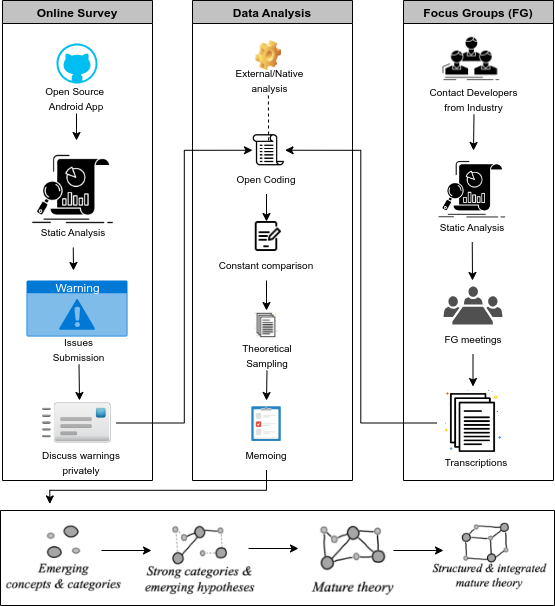
\includegraphics[scale=0.5]{img/metodologia.png}
  \caption{Metodologia adotada no artigo 'Perceptions of Software Practitioners Regarding Crypto-API Misuses and Vulnerabilities'}
  \label{averageWarnings}
\end{figure}


A imagem acima descreve a metodologia utilizada. \cite{perception_developers} A metodologia abordada neste trabalho entra na etapa de 'Análise de Dados' em específico 'Análise externa / nativa', onde é feita a integração dos resultados obtidos pelo LibScout com os contextos fornecidos pelo CryptoGuard e CogniCrypt. Essa integração tenta proporcionar uma visão mais minuciosa e contextualizada de onde as vulnerabilidades identificadas se encontram.
Este trabalho propõe a seguinte integração:

\begin{figure}[!ht]
  \centering
  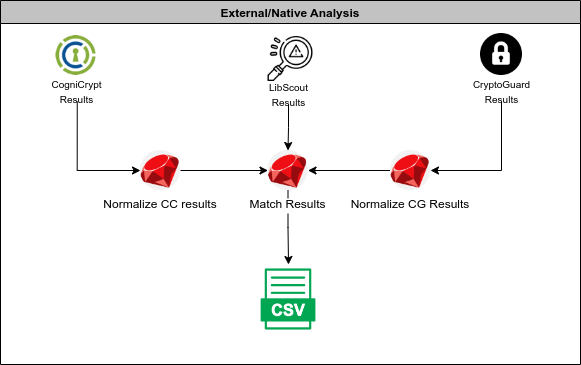
\includegraphics[scale=0.5]{img/studySettingsExternal.png}
  \caption{Metodologia adotada neste trabalho'}
  \label{averageWarnings}
\end{figure}

\begin{itemize}
\item{Coleta de Dados}
A metodologia adotada para a constituição do conjunto de dados envolveu uma cuidadosa seleção de aplicativos Java provenientes do renomado repositório F-Droid. \cite{perception_developers} Este último se destaca como um catálogo de aplicativos de código aberto e livre (FOSS), especialmente concebidos para a plataforma Android.

Nesse processo, buscou-se uma representativa diversidade de categorias de aplicativos, abrangendo áreas vitais como conectividade, finanças, segurança, mensagens de texto (SMS) e funcionalidades de sistema. Tal abordagem foi implementada com o intuito de assegurar uma abrangência abarcadora de contextos e finalidades, enriquecendo assim a robustez e representatividade do conjunto de dados analisado.

\item{Análise Estática}

A etapa subsequente consistiu na aplicação das ferramentas CryptoGuard e CogniCrypt para conduzir uma análise estática detalhada do código fonte dos aplicativos selecionados. Essa abordagem permitiu a identificação minuciosa de possíveis vulnerabilidades relacionadas às APIs criptográficas empregadas nos aplicativos avaliados. O uso dessas ferramentas especializadas proporcionou uma avaliação precisa e abrangente das práticas de segurança adotadas, visando aprimorar a integridade e robustez dos aplicativos em questão.

\item{Identificar a percepção de vulnerabilidade dos desenvoledores}

Após a conclusão da análise estática, foi possível identificar um conjunto de vulnerabilidades que não foram reconhecidas pelos desenvolvedores, bem como aquelas que foram identificadas, porém não receberam intervenção corretiva. Para facilitar a comunicação e o entendimento das questões de segurança identificadas, procedeu-se à criação de GISTS individuais para cada vulnerabilidade.  \cite{perception_developers}  Um GIST é um recurso que permite compartilhar trechos de código, arquivos inteiros ou até mesmo aplicações, e também possibilita a preservação e compartilhamento de saída de console ao executar, depurar ou testar o código. Cada GIST representa um repositório que pode ser clonado ou bifurcado por outras pessoas, promovendo assim a colaboração e a discussão ativa em busca do aprimoramento da segurança nos aplicativos avaliados.

\begin{figure}[!ht]
  \centering
  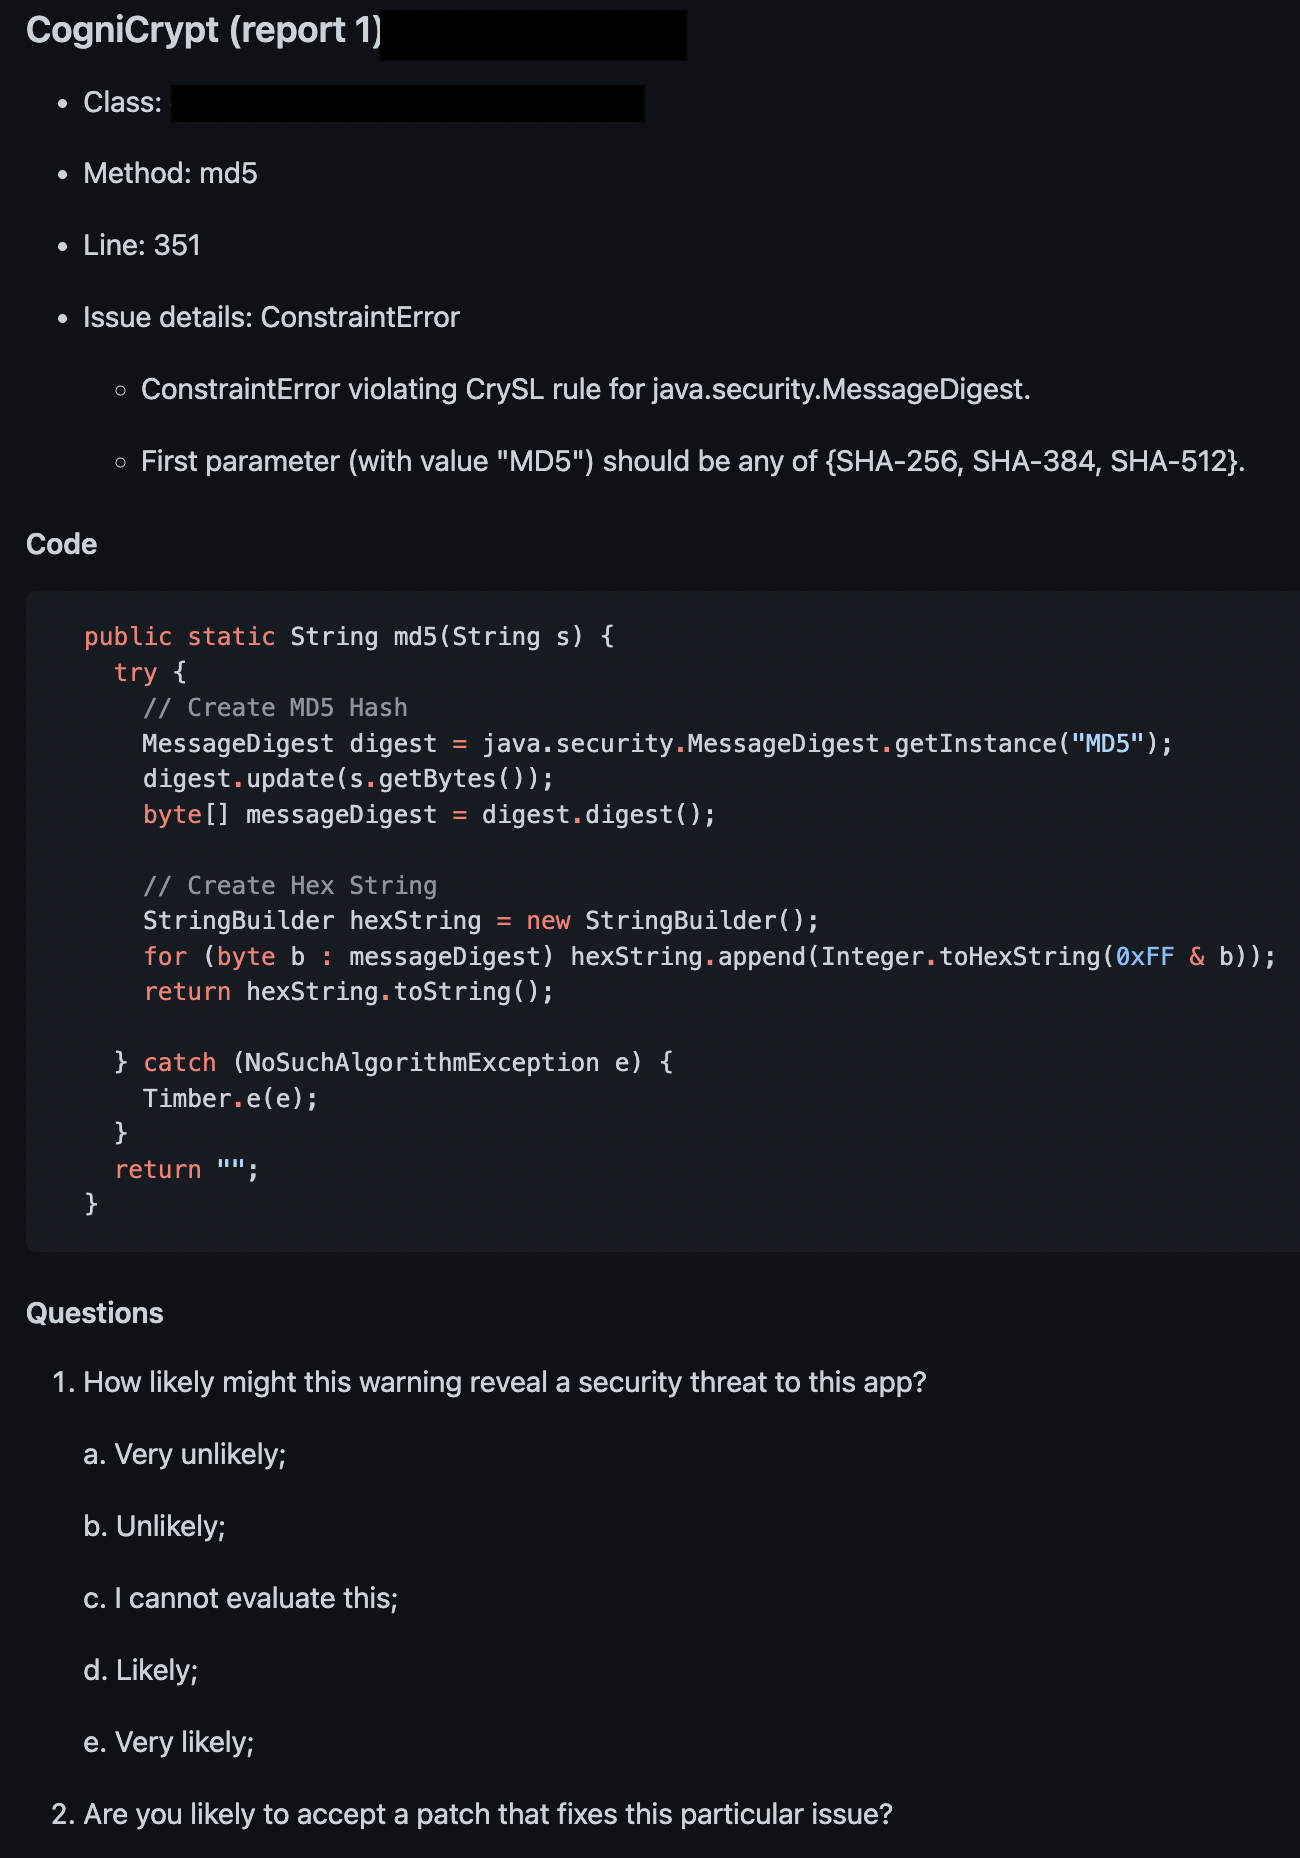
\includegraphics[scale=0.5]{img/gist.png}
  \caption{'Exemplo de uma Gist'}
  \label{averageWarnings}
\end{figure}

\item{Analisar origem das vulnerabilidades}

A etapa seguinte consistiu na análise da origem das vulnerabilidades identificadas. Para realizar essa análise, empregou-se a ferramenta LibScout, a qual desempenhou um papel crucial ao extrair informações detalhadas sobre as APIs criptográficas utilizadas nos aplicativos, permitindo, assim, a identificação de bibliotecas externas empregadas. A utilização do LibScout proporcionou um panorama abrangente das dependências externas dos aplicativos, fornecendo uma visão clara das fontes potenciais de vulnerabilidades no código. Esta abordagem foi essencial para direcionar os esforços na mitigação das ameaças identificadas e fortalecer a segurança das aplicações avaliadas.

A princípio, considerou-se a utilização do LibRadar devido à sua reputação pela rapidez de execução. Contudo, logo se constatou que a ferramenta estava baseada em dados disponibilizados até 2016, o que não condizia com nossa necessidade de informações atualizadas e abrangentes sobre as bibliotecas utilizadas nos aplicativos. Diante dessa constatação, optou-se por descartar o uso do LibRadar e buscar uma alternativa mais alinhada com os objetivos do estudo.


\item{Integração de Resultados}

Foi empreendido um esforço no sentido de desenvolver um processo de integração que possibilitasse a unificação dos resultados obtidos por meio do LibScout com os contextos fornecidos pelo CryptoGuard e CogniCrypt. Essa iniciativa tenta criar uma visão mais abrangente e contextualizada das vulnerabilidades identificadas. Em paralelo, foi realizada uma avaliação da eficácia dessa abordagem, no que tange à habilidade de determinar a origem dos alertas gerados pelas mencionadas ferramentas.

Os dados foram classificados em bibliotecas com warnings, bibliotecas com warnings que definitivamente advém de bibliotecas externas, bibliotecas com warnings que possivelmente advém de bibliotecas externas e total de bibliotecas nativas.

  \begin{itemize}
    \item{Uma biblioteca com warning é o resultado da análise estática da ferramenta seja ela CogniCrypt ou o CryptoGuard.}

    \item{Uma biblioteca com warning que definitivamente advém de bibliotecas externas é o resultado do casamento dos resultados do LibScout com os resultados de uma das duas ferramentas.}

    \item{Uma biblioteca com warning que possivelmente advém de bibliotecas externas é o resultado do casamento dos resultados do LibScout com os resultados de uma das duas ferramentas, porém, ao invés de casar com os resultados finais do LibScout, casamos com o caminho das bibliotecas montadas na árvore de bibliotecas}

    \item{Total de bibliotecas nativas é o total de bibliotecas menos o total de bibliotecas com warning que definitivamente advém de bibliotecas externas e o total de bibliotecas com warning que possivelmente advém de bibliotecas externas.}
  \end{itemize}
\end{itemize}
